\documentclass[aspectratio=169, 10pt, xcolor=table]{beamer}

% --- Package Configuration ---
\usepackage{booktabs}   % Table styling
\usepackage{listings}   % Code blocks
\usepackage{tikz}       % Drawing
\usepackage{multimedia} % Video embedding
\usetikzlibrary{shapes, arrows.meta, positioning, fit, backgrounds, shadows, calc}

% --- Theme Settings: FU Berlin Style ---
\usetheme{Madrid}

% 1. Define FU Berlin Official Colors
\definecolor{FUblue}{RGB}{0, 51, 102}    % Dark Blue (Primary)
\definecolor{FUgreen}{RGB}{153, 204, 0}  % Bright Green (Accent)
\definecolor{FUgray}{RGB}{235, 235, 235} % Light Gray for backgrounds

% 2. Apply Structure Colors
\usecolortheme[named=FUblue]{structure} 

% 3. Specific Overrides for FU Look
\setbeamercolor{frametitle}{bg=FUblue, fg=white}
\setbeamercolor{framesubtitle}{fg=FUgreen}
\setbeamercolor{title}{bg=FUblue, fg=white}
\setbeamercolor{author}{fg=FUblue}
\setbeamercolor{institute}{fg=black}
\setbeamercolor{date}{fg=gray}

\setbeamercolor{block title}{bg=FUblue, fg=white}
\setbeamercolor{block body}{bg=FUblue!5, fg=black}

\rowcolors{2}{FUblue!5}{white}

% --- Custom Colors & Styles ---
\definecolor{codebg}{rgb}{0.95,0.95,0.95}

\lstset{
    backgroundcolor=\color{codebg},
    basicstyle=\ttfamily\footnotesize,
    breaklines=true,
    keywordstyle=\color{FUblue}\bfseries, 
    commentstyle=\color{gray}\itshape,
    stringstyle=\color{FUgreen!80!black},
    frame=single,
    showstringspaces=false,
    escapechar=@
}

\tikzset{
    basicbox/.style={
        rectangle, rounded corners, draw=FUblue!80, fill=white, 
        very thick, align=center, minimum height=0.8cm, drop shadow
    },
    arrow/.style={-{Stealth[length=3mm]}, thick, color=FUblue},
    biarrow/.style={arrows={Stealth[length=3mm]-Stealth[length=3mm]}, thick, color=FUblue},
}

% --- Title Information ---
\title[Smart Home Demo Lab Team 2 Update 4 Report]{Smart Home Demo Lab Team 2 Update 4 Report}
\author[Team 2]{Yixue Wang, Linghao Dong, Yang Xiao, Chenxu Liu, Tong Lu}
\date{January 2026}

\begin{document}

% --- Cover ---
\begin{frame}
    \titlepage
\end{frame}

% ==================== Recap ====================

% --- Slide: Recap - What We've Done ---
\begin{frame}{Recap - Recent Progress}
    {Summary of Work Completed Since Last Update}
    
    \begin{columns}[c]
        \column{0.5\textwidth}
            \onslide<1->{
            \textbf{Frontend}
            \vspace{0.3em}
            \begin{itemize}
                \item Designed \& implemented the \textbf{Homepage}.
                \item Refactored the \textbf{Scene Editor} page.
            \end{itemize}
            
            \vspace{0.5em}
            \textbf{Backend}
            \vspace{0.3em}
            \begin{itemize}
                \item Developed the \textbf{Backend API}.
                \item Built \textbf{Mock Hardware API Server} for testing.
            \end{itemize}
            }

        \column{0.5\textwidth}
            \pause
            \textbf{Infrastructure}
            \vspace{0.3em}
            \begin{itemize}
                \item Optimized \textbf{Database} module.
                \item Improved \textbf{Logging} system.
            \end{itemize}
            
            \vspace{0.5em}
            \textbf{Quality}
            \vspace{0.3em}
            \begin{itemize}
                \item Fixed various \textbf{bugs}.
            \end{itemize}
    \end{columns}
\end{frame}

% ==================== Backend API Implementation ====================

% --- Slide: Backend System - Architecture & Functionality ---
\begin{frame}{Backend System - Architecture \& Functionality}
    {System Design \& Core Capabilities compliant with Specifications}
    
    \begin{columns}[c]
        \column{0.45\textwidth}
            \onslide<1->{
            \textbf{Core Functionality}
            \vspace{0.3em}
            \begin{itemize}
                \item \textbf{Device Lifecycle Management}:
                \begin{itemize}
                    \item Unified CRUD for Equipment \& Sensors.
                    \item Scene Parameter configuration.
                \end{itemize}
                \item \textbf{Automation Engine}:
                \begin{itemize}
                    \item Trigger-Condition-Action logic.
                    \item Dynamic rule enablement.
                \end{itemize}
            \end{itemize}
            }

        \column{0.55\textwidth}
            \pause
            \textbf{Architecture Design}
            \vspace{0.3em}
            \begin{itemize}
                \item \textbf{Strict RESTful Standards}:
                \begin{itemize}
                    \item Resource-oriented URLs (/api/devices/...).
                    \item Standard HTTP verbs (GET, POST, PUT, DELETE).
                \end{itemize}
                \item \textbf{Standardized Response}:
                \begin{itemize}
                    \item Uniform envelopes: \texttt{code}, \texttt{message}, \texttt{data}.
                \end{itemize}
                \item \textbf{Security}: Stateless Bearer Token Authentication.
            \end{itemize}
    \end{columns}
\end{frame}

% --- Slide: Backend System - FastAPI Implementation ---
\begin{frame}[fragile]{Backend System - FastAPI Implementation}
    {High-Performance Implementation Strategy}
    
    \begin{columns}[t]
        \column{0.45\textwidth}
            \onslide<1->{
            \textbf{Technology Stack \& Patterns}
            \vspace{0.3em}
            \begin{itemize}
                \item \textbf{FastAPI Framework}:
                \begin{itemize}
                    \item Native Async I/O support.
                    \item Auto-generated OpenAPI docs.
                \end{itemize}
                \item \textbf{Modular Routing}:
                \begin{itemize}
                    \item \texttt{APIRouter} for domain separation.
                    \item Decoupled endpoints for Devices/Automations.
                \end{itemize}
                \item \textbf{Validation}: Pydantic Models.
            \end{itemize}
            }

        \column{0.55\textwidth}
            \pause
            \textbf{Implementation Logic}
            \vspace{0.3em}
            \begin{itemize}
                \item \textbf{Dependency Injection}:
                \begin{itemize}
                    \item Clean injection of Auth & Service layers.
                    \item Simplifies testing and mocking.
                \end{itemize}
                \item \textbf{Type Safety}:
                \begin{itemize}
                    \item Enforced strict typing for all payloads.
                    \item Automatic validation error handling.
                \end{itemize}
            \end{itemize}
            \vspace{0.5em}
    \end{columns}
\end{frame}

% ==================== Mock Hardware API Server ====================

% --- Slide: Mock Hardware API Server - Overview & Architecture ---
\begin{frame}{Mock Hardware API Server - Overview \& Architecture}
    {Simulates Home Assistant REST API for hardware interface development \& testing}
    
    \begin{columns}[c]
        \column{0.45\textwidth}
            \onslide<1->{
            \textbf{Key Features}
            \vspace{0.3em}
            \begin{itemize}
                \item \textbf{HA-Compatible API} - Full REST endpoints
                \item \textbf{14 Device Types} - Lights, switches, covers, etc.
                \item \textbf{JSON Persistence} - Device state storage
                \item \textbf{FastAPI + Swagger} - Auto documentation
                \item \textbf{Token Auth} - Bearer authentication
            \end{itemize}
            }

        \column{0.55\textwidth}
            \pause
            \textbf{Architecture}
            \vspace{0.3em}
            \centering
            \resizebox{0.95\textwidth}{!}{
            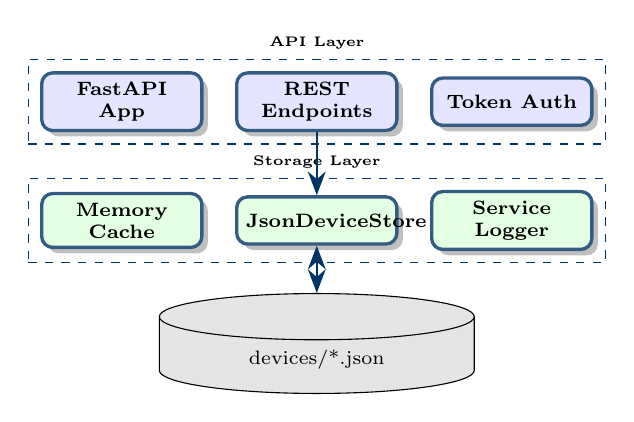
\begin{tikzpicture}[node distance=0.6cm and 0.4cm]
                \tikzstyle{apibox}=[basicbox, fill=blue!10, font=\scriptsize\bfseries, text width=1.8cm, minimum height=0.6cm]
                \tikzstyle{storebox}=[basicbox, fill=green!10, font=\scriptsize\bfseries, text width=1.8cm, minimum height=0.6cm]
                
                % API Layer
                \node[apibox] (app) {FastAPI App};
                \node[apibox, right=of app] (endpoints) {REST Endpoints};
                \node[apibox, right=of endpoints] (auth) {Token Auth};
                \node[fit=(app)(endpoints)(auth), inner sep=0.15cm, draw=FUblue, dashed, label=above:{\tiny\bfseries API Layer}] (l1) {};
                
                % Storage Layer
                \node[storebox, below=0.8cm of endpoints] (store) {JsonDeviceStore};
                \node[storebox, left=of store] (cache) {Memory Cache};
                \node[storebox, right=of store] (logger) {Service Logger};
                \node[fit=(cache)(store)(logger), inner sep=0.15cm, draw=FUblue, dashed, label=above:{\tiny\bfseries Storage Layer}] (l2) {};
                
                % File Layer
                \node[draw, cylinder, shape border rotate=90, aspect=0.3, fill=gray!20, minimum height=0.5cm, minimum width=4cm, below=0.6cm of store, font=\scriptsize] (files) {devices/*.json};
                
                \draw[arrow] (endpoints) -- (store);
                \draw[biarrow] (store) -- (files);
            \end{tikzpicture}
            }
    \end{columns}
\end{frame}

% --- Slide: Mock Hardware API Server - API Endpoints ---
\begin{frame}{Mock Hardware API Server - API Endpoints}
    
    \begin{columns}[t]
        \column{0.48\textwidth}
            \textbf{Core Endpoints}
            \vspace{0.3em}
            
            {\footnotesize
            \begin{tabular}{l l l}
                \toprule
                \textbf{Method} & \textbf{Endpoint} & \textbf{Description} \\
                \midrule
                GET & /api/states & Get all states \\
                GET & /api/states/\{id\} & Get single device \\
                POST & /api/states/\{id\} & Set device state \\
                DELETE & /api/states/\{id\} & Delete device \\
                POST & /api/services/\{d\}/\{s\} & Call service \\
                POST & /api/events/\{type\} & Fire event \\
                GET & /api/config & Get config \\
                \bottomrule
            \end{tabular}
            }
            
            \vspace{0.6em}
            \pause
            \textbf{Helper Endpoints}
            \vspace{0.2em}
            {\footnotesize
            \begin{itemize}
                \item POST /test/reload - Reload devices
                \item GET /test/service-calls - Call history
                \item GET /test/devices/\{domain\} - Filter
            \end{itemize}
            }

        \column{0.52\textwidth}
            \pause
            \textbf{Supported Device Domains}
            \vspace{0.3em}
            
            {\footnotesize
            \begin{tabular}{l l}
                \toprule
                \textbf{Domain} & \textbf{Available Services} \\
                \midrule
                light & turn\_on, turn\_off, toggle \\
                switch & turn\_on, turn\_off, toggle \\
                cover & open, close, set\_position \\
                climate & set\_temperature, set\_hvac\_mode \\
                fan & turn\_on, turn\_off, set\_percentage \\
                lock & lock, unlock \\
                vacuum & start, pause, return\_to\_base \\
                media\_player & play, pause, volume\_set \\
                camera & turn\_on, turn\_off \\
                alarm\_control\_panel & arm\_home, disarm \\
                \bottomrule
            \end{tabular}
            }
    \end{columns}
\end{frame}

% ==================== Development Roadmap ====================

% --- Slide: Development Roadmap ---
\begin{frame}{Development Roadmap}
    {Next Steps Towards Deliverable Demo}
    
    \begin{columns}[c]
        \column{0.5\textwidth}
            \onslide<1->{
            \textbf{This Week}
            \vspace{0.3em}
            \begin{itemize}
                \item \textbf{Scene Editor Adaptation}:
                \begin{itemize}
                    \item Frontend adopted n8n-style DAG design.
                    \item Optimize JSON format for new structure.
                \end{itemize}
                \item \textbf{Backend Execution Logic}:
                \begin{itemize}
                    \item Align automation engine with DAG model.
                \end{itemize}
            \end{itemize}
            }
            
            \vspace{0.8em}
            \pause
            \textbf{Next Week}
            \vspace{0.3em}
            \begin{itemize}
                \item \textbf{End-to-End Testing}:
                \begin{itemize}
                    \item Full integration tests across all layers.
                    \item Validate complete user workflows.
                \end{itemize}
            \end{itemize}

        \column{0.5\textwidth}
            \pause
            \textbf{Goal}
            \vspace{0.3em}
            \begin{block}{Update 5 Target}
                Deliver a \textbf{working demo} of the complete system for the next presentation.
            \end{block}
    \end{columns}
\end{frame}

% ==================== End of Slides ====================

\end{document}
